\begin{figure}[!ht]
  \centering
  \begin{minipage}{.45\textwidth}
    \centering
    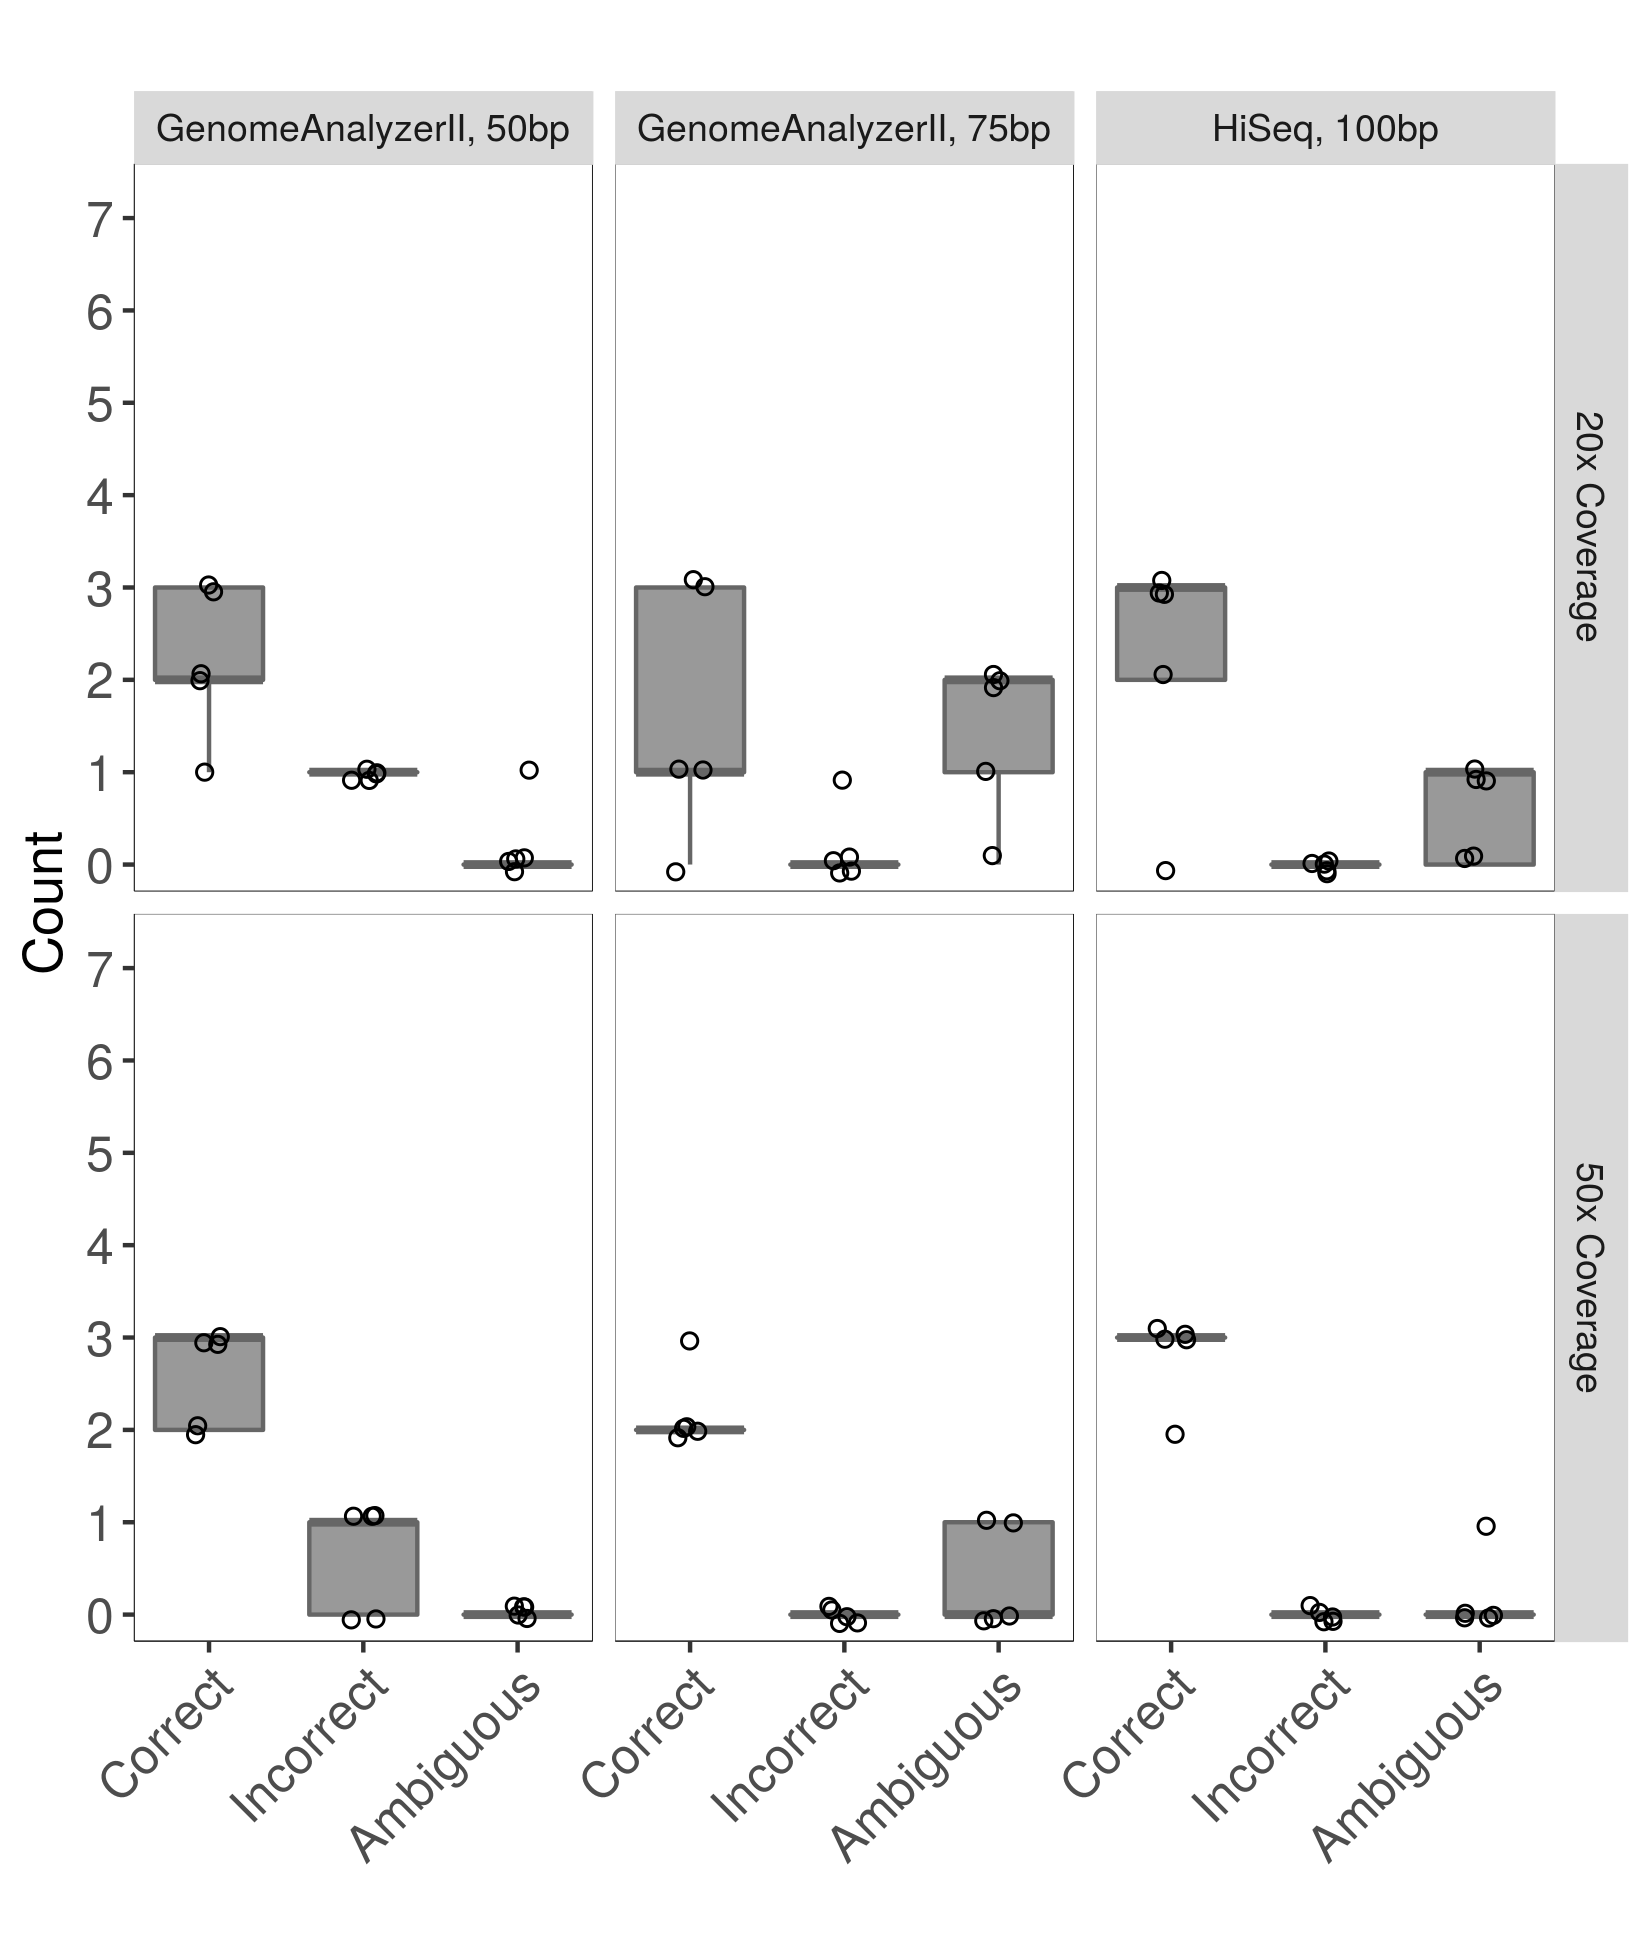
\includegraphics[width=.8\columnwidth]{coli}

    {\footnotesize \textbf{a.} \textit{E. coli} rDNA Assembly}
    \label{fig:sim_coli}
  \end{minipage}

  \begin{minipage}{.45\textwidth}
    \centering
    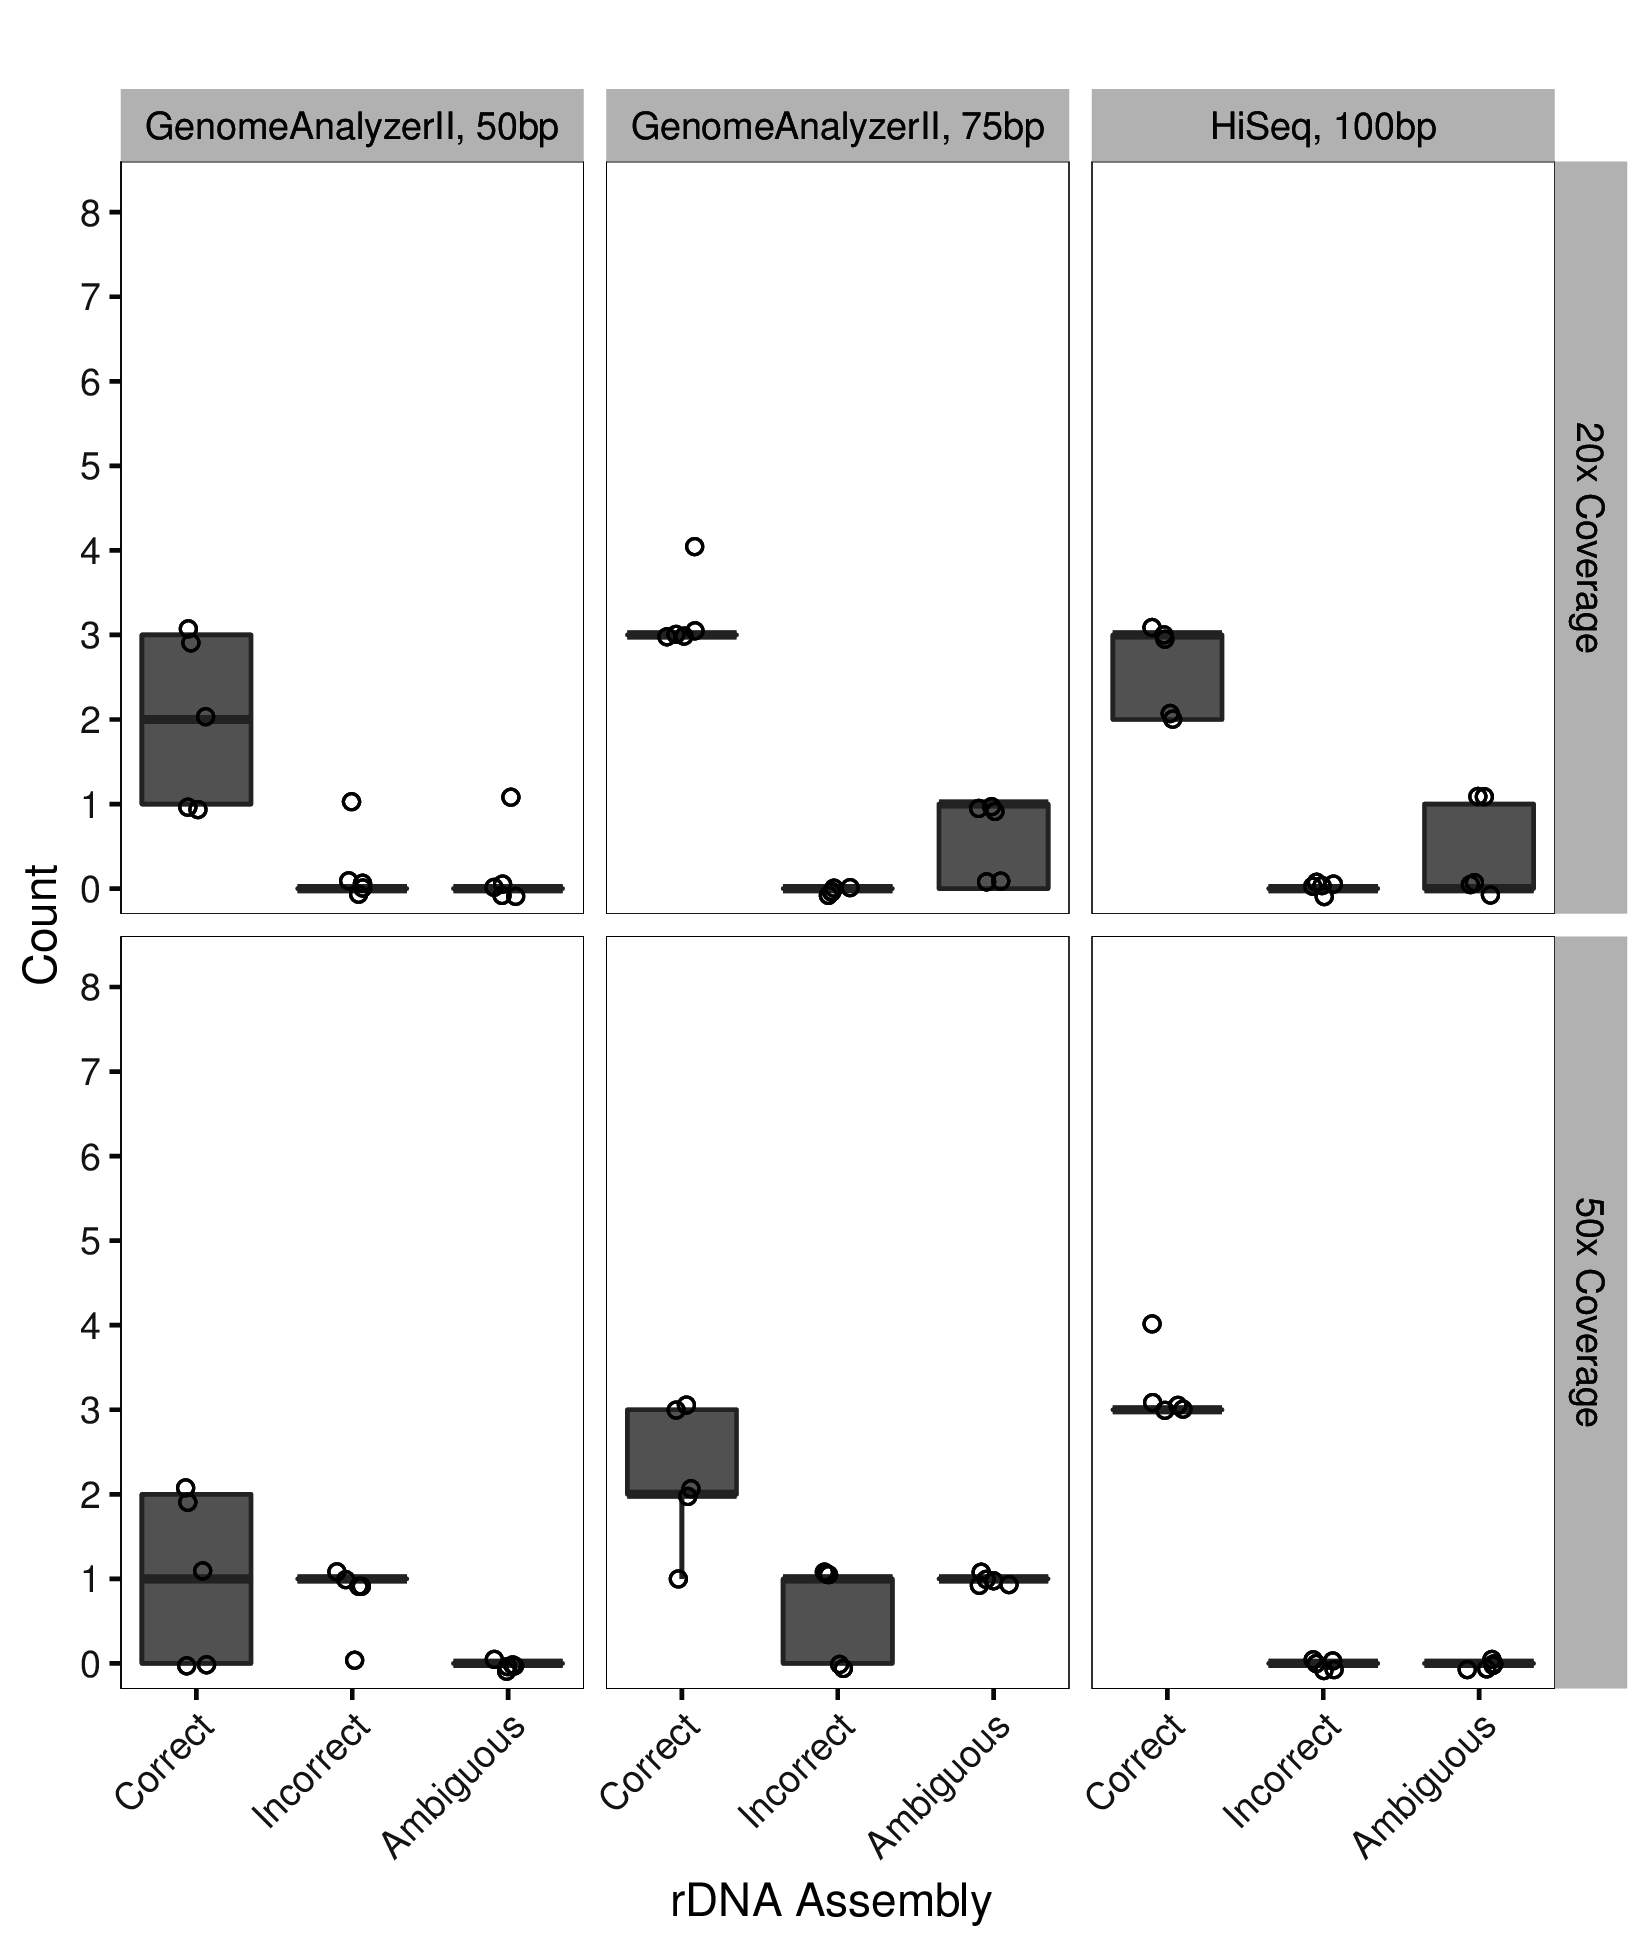
\includegraphics[width=.8\columnwidth]{kleb} %

    {\footnotesize \textbf{b.} \textit{K. pneumoniae} rDNA Assembly}
    \label{fig:sim_kleb}
  \end{minipage}%
  \caption{Comparison of \textit{de fere novo} assemblies of simulated reads generated by pIRS. In most cases, increasing coverage depth and read length resulted in fewer misassemblies. Assemblies were scored using \texttt{score}; the y axis reflects the total number of rDNAs in the genome (7 and 8 rDNAs, for \textit{E. coli} and \textit{K. pneumoniae} respectively). The (n=9) assemblies shown for each genome are the result of differently seeded read simulations.}
  \label{fig:simreads}
\end{figure}
